
%% Creator David Li
% Modified matlab xsl latex template file to suit needs
% This LaTeX was auto-generated from an M-file by MATLAB.
% To make changes, update the M-file and republish this document.

\documentclass[12pt]{scrartcl}
\nonstopmode

\title{Matlab}
\usepackage[utf8]{inputenc}
\usepackage{graphicx}
\usepackage{epstopdf}
\usepackage{color}
\usepackage{xcolor}
\usepackage{amsmath}
\usepackage[ocgcolorlinks]{hyperref}
\usepackage{bookmark}
\usepackage[hmargin=2cm,vmargin=2.5cm]{geometry}
\usepackage{fancyhdr}
\usepackage{booktabs}
\sloppy
\definecolor{lightgray}{gray}{0.5}
% \definecolor{myText}{HTML}{2B2B2B}
\definecolor{fontColor}{HTML}{171717}
\setlength{\parindent}{0pt}

\makeindex

\usepackage{listings}
\definecolor{mygreen}{RGB}{28,172,0} % color values Red, Green, Blue
\definecolor{mylilas}{RGB}{170,55,241}
\lstset{language=Matlab,%
	%basicstyle=\color{red},
	breaklines=true,%
	morekeywords={matlab2tikz},
	keywordstyle=\color{blue},%
	morekeywords=[2]{1}, keywordstyle=[2]{\color{black}},
	identifierstyle=\color{black},%
	stringstyle=\color{mylilas},
	commentstyle=\color{mygreen},%
	showstringspaces=false,%without this there will be a symbol in the places where there is a space
	%numbers=left,%
	%numberstyle={\tiny \color{black}},% size of the numbers
	%numbersep=9pt, % this defines how far the numbers are from the text
	emph=[1]{for,end,break},emphstyle=[1]\color{red}, %some words to emphasise
	%emph=[2]{word1,word2}, emphstyle=[2]{style},  
    captionpos=b,
    caption={Matlab Code Snippet:},
}
\usepackage{tcolorbox}
\tcbuselibrary{listings}
\tcbuselibrary{breakable}


\newtcblisting[auto counter,number within=section*]{matlaboutput}[2][]{sharp corners, breakable,
    fonttitle=\bfseries,colback=white, colframe=black!90, listing only, 
    listing options={language=Matlab, showstringspaces=false, breakatwhitespace=true, breaklines=true, tabsize=4}, 
    title=Matlab Output \thetcbcounter: #1} 

%\usepackage{fancyhdr} 
%\fancyhf{}
%\cfoot{\thepage}
%\pagestyle{fancy}

\begin{document}

\begin{center}
	\hrule
	\vspace{.4cm}
	{\textbf { \large ELEC 460 --- Control Theory II}}
\end{center}
{\textbf{Name:}\ David Li \hspace{\fill} \textbf{Student Number:}} \ V00818631  \\
{\textbf{Due Date:} Thursday, 11 January 2018, 11:30 AM \hspace{\fill} \textbf{Assignment:} Number 1 \\
	\hrule
	
	
	
	%\tableofcontents
	%\newpage
	
	
	%\subsection*{ELEC 460 Assignment 1}
	%%{toc}{subsection}{ELEC 460 Assignment 1}
	%\phantomsection
	%
	%
	%\begin{lstlisting}[language = Matlab,frame=single,caption={}]
	%clear all
	%close all
	%\end{lstlisting}
	
	
	\subsection*{1. Sketch the root locus}
	%{toc}{subsection}{1. Sketch the root locus}
	\phantomsection
	
	
	\begin{lstlisting}[language = Matlab,frame=single,caption={}]
	G1 = zpk([],[0,-1,-20],20) % create transfer function
	figure(1); rlocus(G1) % Plot root locus
	\end{lstlisting}
	
	
	% \begin{matlaboutput}{}
	%G1 =
	% 
	%        20
	%  --------------
	%  s (s+1) (s+20)
	% 
	%Continuous-time zero/pole/gain model.
	%
	%\end{matlaboutput}
	
	\begin{figure}[h]
		\centering
		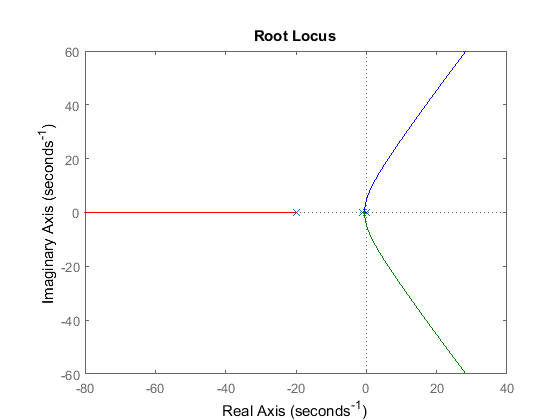
\includegraphics [width=0.7\linewidth]{ELEC460A1_01.png}
		\caption{Root Locus when K =1}
		%\caption{}
		% Alternative is to typeset the caption myself, which makes more sense to me.
		% \label{$fig:ELEC460A1_01.png$}
	\end{figure}
	
	
	\subsection*{2. Find Kv.}
	%{toc}{subsection}{2. Find Kv.}
	\phantomsection
	Using the final value theorem: $x(\infty ) = \mathop {\lim }\limits_{s \to 0} sX(s)$ \newline 
	
	\begin{lstlisting}[language = Matlab,frame=single,caption={}]
	syms s ;Kv = limit(s*20/(s*(s+1)*(s+20)),s,0)% compute Kv using limits
	\end{lstlisting}
	
	
	% \begin{matlaboutput}{} 
	%Kv =
	% 
	%1
	% 
	%\end{matlaboutput}
	
	
	\subsection*{3. Sketch Bode and Nyquist plots.}
	%%{toc}{subsection}{3. Sketch Bode and Nyquist plots.}
	%\phantomsection
	
	
	\begin{lstlisting}[language = Matlab,frame=single,caption={}]
	figure(2); bode(G1)
	figure(3); nyquist(G1)
	\end{lstlisting}
	
	\begin{figure}
		\centering
		\begin{minipage}{0.5\textwidth}
			\centering
			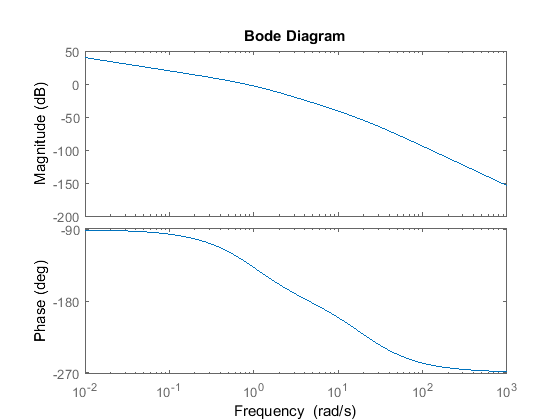
\includegraphics [width=1\linewidth]{ELEC460A1_02.png} % first figure itself
			\caption{Bode plot when K=1}
		\end{minipage}\hfill
		\begin{minipage}{0.5\textwidth}
			\centering
			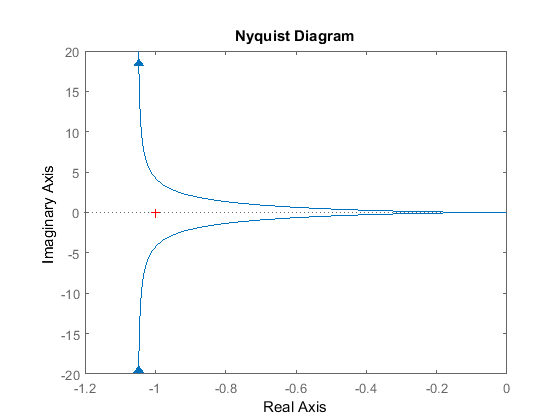
\includegraphics [width=1\linewidth]{ELEC460A1_03.png} % second figure itself
			\caption{Nyquist plot when K=1}
		\end{minipage}
	\end{figure}
	
	\subsection*{4. Find K so that $\zeta=\sqrt(2)/2$ for the closed loop system.}
	%%{toc}{subsection}{4. Find K so that zeta=sqrt(2)/2 for the closed loop system.}
	%\phantomsection
	
	% Consider deleting the zeta value computing and the fprintf
	%\begin{lstlisting}[language = Matlab,frame=single,caption={}]
	%zeta = sqrt(2)/2
	%figure(4);
	%gains = -1:0.00125:1;
	%rlocus(G1,gains); sgrid; K = 0.476;
	%% Plot test box with results onto plot
	%gainString = ['Gain: ' num2str(K)];text(-0.25,0.5,gainString);
	%fprintf('Using the root locus the value K at which zeta is 0.7071 is: %0.3f. \n', K )
	%\end{lstlisting}
	
	% Rewrite using latex commands   
	% \begin{matlaboutput}{}
	%zeta =
	%
	%    0.7071
	%
	%Using the root locus the value K at which zeta is 0.7071 is: 0.476. 
	%\end{matlaboutput}
	% I think I might remove this picture
	Using the root locus the value K at which $\zeta$ is 0.7071 is: 0.476. 
	%\begin{figure}[h]
	%	\centering
	%	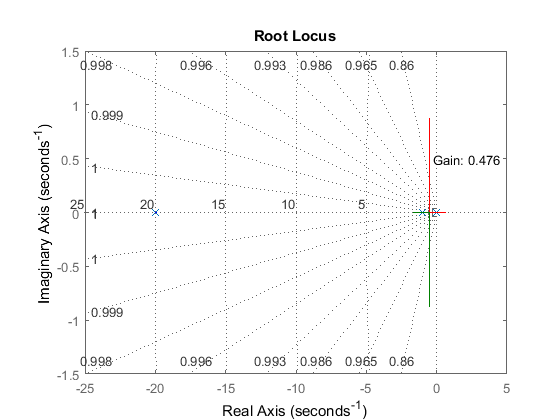
\includegraphics [width=0.7\linewidth]{ELEC460A1_04.png}
	%	\caption{$ELEC460A1_04.png$}
	%	%\caption{}
	%	% Alternative is to typeset the caption myself, which makes more sense to me.
	%	% \label{$fig:ELEC460A1_04.png$}
	%\end{figure}
	
	
	\subsection*{5. Find phase and gain margins for this K.}
	%%{toc}{subsection}{5. Find phase and gain margins for this K.}
	%\phantomsection
	
	
	\begin{lstlisting}[language = Matlab,frame=single,caption={}]
	G1new = zpk([],[0,-1,-20],20*K)
	figure(5); margin(G1new)
	\end{lstlisting}
	
	\begin{figure}[ht]
		\centering
		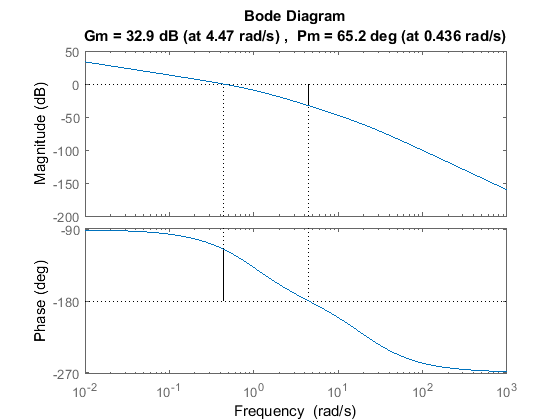
\includegraphics [width=0.7\linewidth]{ELEC460A1_05.png}
		\caption{Phase and Gain Margin in Bode Plot}
		%\caption{}
		% Alternative is to typeset the caption myself, which makes more sense to me.
		% \label{$fig:ELEC460A1_05.png$}
	\end{figure}
	
	As shown in the updated bode plot, the $PM=65.2^o$ and has a $GM=32.9 \text{DB}$
	\subsection*{6. Sketch the step and ramp responses of the closed loop system for this K}
	%%{toc}{subsection}{6. Sketch the step and ramp responces of the closed loop system for this K}
	%\phantomsection
	
	
	\begin{lstlisting}[language = Matlab,frame=single,caption={}]
	G1tfnew = tf(G1new)
	subplot(2,1,1); step(G1tfnew); %% create subplot for step function
	ramps = tf([1,0],[1]);
	subplot(2,1,2); step(G1tfnew/ramps); %% create subplot for ramp function
	\end{lstlisting}
	
	
	% \begin{matlaboutput}{}
	%G1tfnew =
	% 
	%         9.52
	%  -------------------
	%  s^3 + 21 s^2 + 20 s
	% 
	%Continuous-time transfer function.
	%
	%\end{matlaboutput}
	
	\begin{figure}[ht]
		\centering
		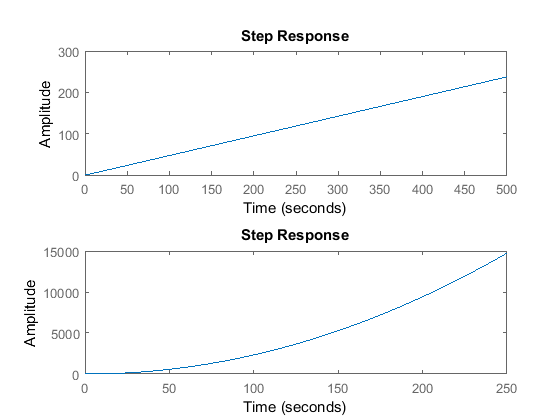
\includegraphics [width=0.7\linewidth]{ELEC460A1_06.png}
		\caption{Step Response of Transfer function with K = 0.479}
		%\caption{}
		% Alternative is to typeset the caption myself, which makes more sense to me.
		% \label{$fig:ELEC460A1_06.png$}
	\end{figure}
	
	
	\subsection*{7. Discuss the connection between Kv, zeta, margins and the response of the closed loop system.}
	%{toc}{subsection}{7. Discuss the connection between Kv, zeta, margins and the response of the closed loop system.}
	
	
	
	The value of Kv is 1, so the steady state velocity error is constant. Additionally 
	the system is stable because of a positive phase and gain margin. Finally, the value of 
	$\zeta = 0.7071$ corresponds to a gain of 0.427.   \newline
    


\end{document}
    
